\begin{frame}
    \frametitle{Markdown}

    Markdown is a simple markup language for creating \textbf{formatted text} designed to be easily readable in
    its source code form.
    \medskip

    \pause
    \begin{columns}
        \begin{column}[T]{.45\textwidth}
            Hugo takes Markdown...\ \\
            \smallskip
            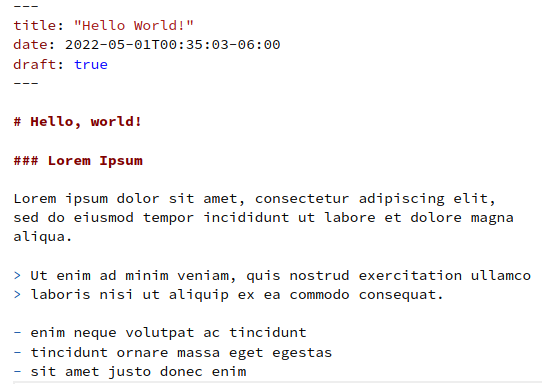
\includegraphics[width=\textwidth]{images/markdown.png}
        \end{column}
        \pause
        \begin{column}[c]{.1\textwidth}
            $$ \to $$
        \end{column}
        \begin{column}[T]{.45\textwidth}
            ...and turns it into a webpage:\ \\
            \smallskip
            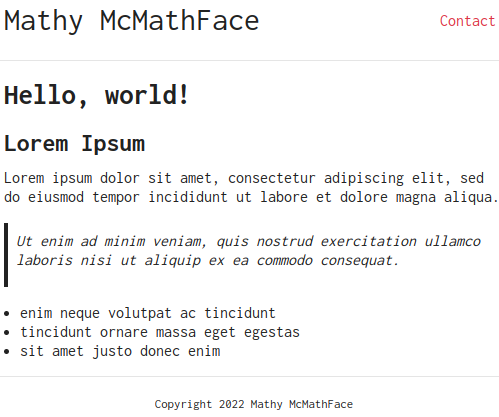
\includegraphics[width=\textwidth]{images/rendered_markdown.png}
        \end{column}
    \end{columns}

    \pause
    \vfill

    In many ways, Hugo does for webpages what \LaTeX \: does for documents.
    
\end{frame}